
\section{Grundlagen}

In diesem Kapitel sollen einige Grundlagen erklärt werden. Zunächst wird erklärt, was genau Websockets sind. Dann wird auf die Technologie Groovy on Grails näher eingegangen. Anschließend wird das Spring Framework beleuchtet, bevor es dann eine Erläuterung bezüglich SockJS und Stomp gibt.

\subsection{Websockets}\label{websocket}

Websockets erlauben eine Full-Duplex single-socket Verbindung. Zwischen dieser Verbindung können Nachrichten zwischen einem Server und einem Client ausgetauscht werden. 

Ursprünglich musste z. B. ein Client bei einem Server polling betreiben, das heißt immer wieder bei einem Server nachfragen, ob relevante Informationen für den Client vorhanden sind. Ein Websocket stellt eine Bidirektionale Verbindung her, welches das polling nicht mehr notwendig macht \cite[Seite 751f]{iuliana2017}. Daten können zwischen dem Client und dem Server gleichzeitig hin und her geschickt werden. Eine Websocket Verbindung zwischen Client und Server ist persistent \cite{malte2017}. 

\subsection{Groovy}

Groovy ist eine Programmiersprache unter der Apache-Lizenz \cite{groovy2017}.
Es wurde für die Java Plattform entwickelt, um die Entwicklung von Anwendungen zu beschleunigen. Zudem war eines der Ziele, dass die Syntax vertraut ist und einfach zu lernen. Zudem sit es mit anderen Java Programmen Kompatibel. 

Grooy ist sowohl eine kompilierte, als auch eine Interpretierte Programmiersprache. 
Listing \ref{listingGb} zeigt ein einfaches Beispiel eines Groovy Programms. Es wird eine einfache Klasse angelegt mit verschiedene Attribute. Dabei ist zu sehen, dass nicht zwingend der Konkrete Datentyp angegeben werden muss. Es besteht die Möglichkeit den Datentyp mit \textit{def} anzugeben, so dass der Datentyp des Attributes automatisch ermittelt wird, je nachdem was das Attribute für einen Wert zugewiesen bekommt. 

In der Groovy Dokumentation \cite{groovylang2017} ist die Sprache Groovy beschrieben.

\begin{lstlisting}[language=Groovy,caption={Eine einfache Groovy Klasse}, label=listingGb]
class Person{ 
	
	def vorname = 'Max'
	String name = 'Mustermann'
	int alter = 42
	
	def printName(){

		println name
		
	}
}

def person = new Person()

person.printName()
\end{lstlisting}

\subsection{Grails}

Grails ist eine Groovy basierte Webtechnologie, welche auf die \ac{JVM} läuft. Grails setzt dabei auf Spring auf \cite{grails2017}. Grails erlaubt das erstellen von Web Anwendungen innerhalb kürzester Zeit. Zudem unterstützt Grails Scaffolding, was das Generieren von CRUD Pages ermöglicht. Grails basiert zudem auf das \textit{convention over configuration} Prinzip. 

Grails nutzt das JavaEE als Grundlage für die Architektur und Spring für die Strukturierung der Anwendung via \textit{dependency injection}. Zudem nutzt Grails Gradle \cite{grailsVogella2017}. Abbildung \ref{grailsarchi} gibt einen Einblick in Grails Architektur.

\begin{figure*}[h]
  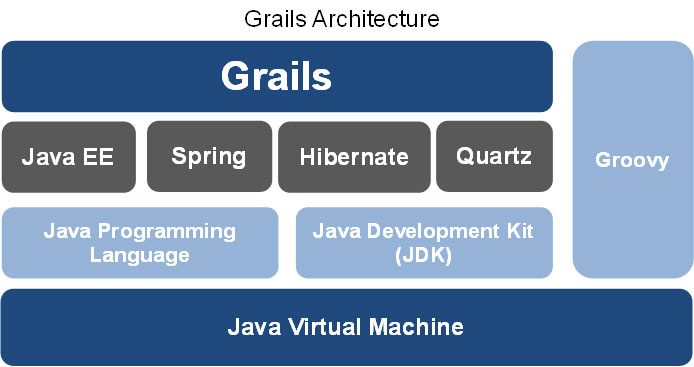
\includegraphics[width=\textwidth,height=7cm]{grailsarchitecture.jpg}
  \caption{Grails Architektur \protect\footnotemark}
  \label{grailsarchi}
\end{figure*}
\footnotetext{https://www.dunebook.com/wp-content/uploads/2017/02/Grails-Architecture1.jpg}%s%s

\subsection{Spring}\label{spring}

Bei Spring handelt es sich um ein plattformunabhängiges Framework, welches unter der Apache-Lizenz von  SpringSource \footcite{https://spring.io/} veröffentlicht wurde. Da Spring selber in Java geschrieben ist, ist es zu Groovy kompatible. Mithilfe von Spring soll das entwickeln von Java/J2EE Anwendungen vereinfacht werden, zudem soll die Entwicklung auch Produktiver vonstatten gehen \cite[Seite 1]{johnson2005}. 

Spring ermöglicht es, dass Anwendungen für viele verschiedene Zwecke geschrieben werden. So ist es möglich Anwendungen sowohl für Applets zu Entwickeln, als auch für standalone Clients. Das half Spring dabei sich gegenüber der Konkurrenz zu behaupten. Spring ist eines der meist genutzten leichtgewichtigen Frameworks. 
Einige Merkmale von Spring sind \cite[Seite 5]{johnson2005}:

\begin{itemize}
\item Inversion of Control:\\ Der core Container von Spring bietet Konfigurationsmanagement für \ac{POJO} Dateien. POJOs sind einfache Java Objekte, die möglichst wenig externe Abhängigkeiten haben. 
\\
\item Aspektorientierte Programmierung:\\ Spring bietet für die Aspektorientierte Programmierung wichtige out-of-the-box Service an, wie z. B. deklaratives Transaktionsmanagement.
\\
\item Transaktionsmanagement:\\ Spring bietet eine Abstraktion von einer Transaktion, welches auf \ac{JTA} aufsetzt.
\\
\item MVC Web Framework:\\ Spring bietet ein flexibles Request basiertes MVC Web Framework. 
\\
\item Leichtgewichtiger Fernzugriff:\\ Spring bietet Unterstützung für POJO basierte Fernzugriffe mithilfe von Protokollen, wie RMI, IIOP, Hessian oder anderen Webservice Protokolle.
\end{itemize}

Mit Version 4.0 unterstützt Spring auch die Anforderung JSR-356 \cite[Seite 14]{iuliana2017}. JSR-356 ist die Java Spezifikation für Websockets\footnote{https://www.jcp.org/en/jsr/all}. Websockets werden in \ref{websocket} näher erläutert.


\subsection{SockJS}

SockJS ist eine Browser JavaScript Bibliothek. Es bietet ein Websocketartiges Objekt an. Die JavaScript Bibliothek bietet eine Kommunikationschannel zwischen Browser und Webserver an, welches wenig Latenzzeit hat \cite{sockjs}.

\subsection{Stomp}

Bei Stomp handelt es sich um ein einfaches Textorientiertes Nachrichten Protokoll. Jeder Stomp Client kann mit einem Stomp Nachrichten Broker Kommunizieren. So können unterschiedliche Systeme miteinander Kommunizieren \cite{stomp}.

\section{Websocket mit Grails}

In diesem Kapitel gibt es ein Überblick über die Implementierung eines Websockets mit Grails. Zunächst werden die relevanten Annotationen eingeführt. Anschließend wird erklärt, wie der HTML Code des Clients aussehen kann. Darauf aufbauend wird dann der Quellcode des Servers erklärt. 

--TODO--

Um in Grails über Websockets zu kommunizieren, muss folgende Zeile in build.gradle unter den \textit{Depenencies} eingefügt werden\footnote{https://plugins.grails.org/plugin/zyro/grails-spring-websocket}.\\
\textit{compile 'org.grails.plugins:grails-spring-websocket:2.3.0'}\\
\\

\subsection{Annotationen}\label{ankapitel}

Da bei der Websocket Programmierung in Grails, die Bibliothek Spring \ref{spring} genutzt wird, wird auch von dessen Annotationen starken Gebrauch gemacht. Folgend werden die wichtigsten Annotationen, die für die Websocket Programmierung mit Grails benötigt werden, aufgelistet und erklärt \cite{spring2017}

\begin{itemize}
	\item @Controller:\\	
	Diese Annotation zeichnet eine Klasse als Controller aus. In Grails ist diese Angabe Optional.
	
	\item @MessageMapping:\\
	Diese Annotation ruft die annotierte Methode auf, wenn eine Nachricht zur angegebenen Stelle versendet wird. In Listing \ref{messagmap} wird die Methode \textit{sendMessage} dann aufgerufen, wenn eine Nachricht an \textit{/destination} gesendet wird. 
	   
	\item @SendTo:\\
	Diese Annotation sorgt dafür, dass alle Clients, welche die angegebene Stelle 	abonniert haben, den Wert, denn die Methode \textit{getGreeting} zurück gibt, auch erhalten. In Listing \ref{sendto} werden alle Clients die Nachricht \textit{Hallo user} erhalten, wenn sie \textit{/topic/destination} abonniert haben. 
    
    
\end{itemize} 

\begin{lstlisting}[language=Groovy,caption={Beispiel von @MessageMapping}, label=messagmap]
import org.springframework.messaging.handler.annotation.MessageMapping

class MessageMappingExampleController {

    @MessageMapping("/destination")
    protected String sendMessage(String message){

    	return message;
    }
}
\end{lstlisting}

\begin{lstlisting}[language=Groovy,caption={Beispiel von @SendTo}, label=sendto]
import org.springframework.messaging.handler.annotation.MessageMapping
import org.springframework.messaging.handler.annotation.SendTo

class SendToExampleController {
  
	@MessageMapping("/destination")
	@SendTo("/topic/destination")
    protected String getGreeting(String message){

    	return "Hallo user";
    }
}
\end{lstlisting}

\begin{lstlisting}[language=Groovy,caption={Beispiel von @Controller}, label=controller]
import org.springframework.stereotype.Controller

@Controller
class ExampleController { }
\end{lstlisting}

\subsection{Quellcode des Clients}\label{clientKapitel}

Damit der Client über den Websocket mit dem Server Kommunizieren kann, benötigt dieser ein Objekt vom Typ SockJS, dass als Socket dient, über dass Kommuniziert wird. Zudem ist auch das Protokoll Stomp notwendig. In Listing \ref{listingClient} ist der Code eines \ac{GSP} Dokuments zu sehen. Hier wird mithilfe der Grails Methode createLink\footnote{http://docs.grails.org/3.2.3/ref/Tags/createLink.html} eine \ac{URI} generiert, auf.
Mithilfe des Sockets wird ein Stomp Objekt generiert. Anschließend wird mit der Methode connect\footnote{https://stomp-js.github.io/stomp-websocket/codo/class/Client.html\# connect-dynamic} der Client einen Asynchronen Aufruf tätigen. In dieser wird festgelegt, was der Client abonniert, in diesem Fall \textit{/topic/hello}. 
Anschließend wird das verhalten definiert, was beim drücken eines Buttons passieren soll.
Die dargestellte Seite stellt dem Nutzer nur einen Button zur Verfügung, welche beim drauf klicken eine Nachricht in eine Div-box einfügt. 

\begin{lstlisting}[language=HTML,caption={GSP Code des Clients}, label=listingClient]

<!DOCTYPE html>
<html>
<head>
    <meta name="layout" content="main"/>

    <asset:javascript src="application"/>
    <asset:javascript src="spring-websocket"/>

    <script type="text/javascript">
        $(function () {
        
            var socket = new SockJS("${createLink(uri: '/stomp')}");
            var client = Stomp.over(socket);

            client.connect({}, function () {
                client.subscribe("/topic/hello", function (message) {
                    $("#textbox").append(message.body);
                });
            });

            $("#examplebutton").click(function () {
                client.send("/app/hello", {}, "Beispiel Nachricht ");
            });
        });
    </script>
</head>

<body>
<button id="examplebutton">Button</button>

<div id="textbox"></div>
</body>
</html>

\end{lstlisting}

\subsection{Quellcode des Servers}

Der Quellcode auf der Server Seite ist sehr simple. Für ein einfach Beispiel reichen die Annotationen aus dem Kapitel \ref{ankapitel}. In diesem Beispiel Quellcode wird die Methode \textit{Message} dann aufgerufen, wenn eine Nachricht an \textit{/hello} erfolgt. Anschließend wird die Methode ausgeführt, bis sie dann alle Abonnenten den Wert übermittelt, denn diese Methode liefert. 
In diesem Quellode wird mit dem drücken des Buttons aus \ref{clientKapitel} dafür gesorgt, dass eine Nachricht sowohl versendet, als auch empfangen wird.

\begin{lstlisting}[language=Groovy,caption={Beispiel der Controller Klasse}, label=listingexampleControllerClass]

import org.springframework.messaging.handler.annotation.MessageMapping
import org.springframework.messaging.handler.annotation.SendTo

class ExampleController {
	
	@MessageMapping("/hello")
	@SendTo("/topic/hello")
	protected String Message(String message) {
		return "${message}"
	}	
}
\end{lstlisting}


